\documentclass[../main.tex]{subfiles}

\addbibresource{\subfix{../references.bib}}

\begin{document}

\ifSubfilesClassLoaded{%
    \setcounter{chapter}{8}%
    \begin{refsection}
}{}

\chapter{Local Optimization dan Data Flow Analysis}
\label{chap:local-optimization}

\begin{subcpmk}
  \item \textbf{Sub-CPMK 4.3:} Menganalisis dan mengoptimasi kode tingkat lokal
\end{subcpmk}

% ============================================================
% MATERI POKOK
% ============================================================
\section{Kerangka Kerja Data-Flow Analysis}

\compiler{Data-Flow Analysis (DFA)} adalah proses pengumpulan informasi tentang aliran data melalui graf kendali alir (\textit{Control Flow Graph}) \cite{nguyen2024semantic}. Informasi ini digunakan untuk menjawab pertanyaan global seperti: "Apakah variabel $x$ pasti memiliki nilai 10 di baris ini?" atau "Apakah nilai $y$ akan dibaca lagi di masa depan?".

\subsection{Iterative Data-Flow Framework}
Untuk menyelesaikan masalah DFA secara sistematis, kita menggunakan kerangka kerja iteratif. Setiap algoritma DFA dapat didefinisikan dengan empat komponen utama:
\begin{enumerate}
    \item \textbf{Direction}: Arah aliran (\textit{Forward} atau \textit{Backward}).
    \item \textbf{Domain}: Himpunan nilai yang dianalisis (misal: himpunan definisi variabel atau ekspresi).
    \item \textbf{Transfer Function} ($f_B$): Aturan bagaimana sebuah blok mengubah informasi data-flow. Format umumnya: $OUT[B] = f_B(IN[B])$.
    \item \textbf{Meet operator} ($\wedge$): Aturan penggabungan informasi ketika dua atau lebih jalur dalam CFG bertemu (biasanya berupa \textit{Union} $\cup$ atau \textit{Intersection} $\cap$).
\end{enumerate}

\subsection{Representasi Bit-Vector}
Agar proses DFA berjalan cepat, kompilator biasanya menggunakan representasi \textbf{Bit-Vector}. Setiap elemen dalam domain direpresentasikan oleh satu bit dalam sebuah \textit{array of bits}. 
\begin{itemize}
    \item Bit $1$ berarti properti tersebut \textit{true} atau ada dalam set.
    \item Bit $0$ berarti \textit{false} atau tidak ada.
\end{itemize}
Dengan bit-vector, operasi set seperti \texttt{Union} dapat dilakukan menggunakan instruksi bitwise \texttt{OR} ($|$), dan \texttt{Intersection} menggunakan bitwise \texttt{AND} ($\&$), yang didukung sangat cepat oleh perangkat keras CPU.

\begin{figure}[!htbp]
    \centering
    \adjustbox{max width=0.8\textwidth,center}{%
    \begin{tikzpicture}[
        node/.style={rectangle, draw=blue!50, fill=blue!10, font=\small, align=center, rounded corners, minimum height=0.8cm},
        arrow/.style={->, >=stealth, thick}
    ]
    \node[node] (in) {IN[B]};
    \node[node, right=1.5cm of in] (bb) {Basic Block $B$};
    \node[node, right=1.5cm of bb] (out) {OUT[B]};
    \draw[arrow] (in) -- (bb);
    \draw[arrow] (bb) -- node[above, font=\footnotesize] {$f_B$} (out);
    \end{tikzpicture}%
    }
    \caption{Model Aliran Data pada Satu Basic Block}
\end{figure}

\section{Reaching Definitions Analysis}

Analisis \compiler{Reaching Definitions} adalah analisis \textbf{Forward} dengan meet operator \textbf{Union} ($\cup$). Analisis ini menentukan definisi (penugasan nilai) mana yang mungkin masih aktif saat mencapai titik program tertentu.

\subsection{Persamaan Aliran Data}
Untuk setiap blok $B$, hubungannya didefinisikan sebagai:
\begin{enumerate}
    \item \textbf{Meet Operation}: $IN[B] = \bigcup_{P \in Pred(B)} OUT[P]$ (Definisi yang mencapai awal blok adalah gabungan dari semua yang keluar dari pendahulunya).
    \item \textbf{Transfer Function}: $OUT[B] = GEN[B] \cup (IN[B] - KILL[B])$.
\end{enumerate}

Di mana:
\begin{itemize}
    \item $GEN[B]$: Himpunan definisi yang dibuat di dalam blok $B$ dan mencapai akhir $B$.
    \item $KILL[B]$: Himpunan definisi di luar $B$ yang variabelnya di-assign ulang di dalam $B$.
\end{itemize}

\subsection{Konsep Fixed-Point}
Kompilator menjalankan algoritma ini secara berulang di seluruh CFG. Karena himpunan data hanya bisa bertambah (monotonik) dan jumlah definisi terbatas, algoritma dijamin akan berhenti pada suatu titik di mana nilai $IN$ dan $OUT$ tidak lagi berubah. Titik stabil ini disebut \textbf{Fixed-Point}.

\begin{figure}[!htbp]
    \centering
    \adjustbox{max width=0.8\textwidth,center}{%
    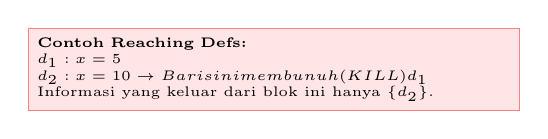
\begin{tikzpicture}[
        rect/.style={rectangle, draw=red!50, fill=red!10, text width=6cm, font=\tiny}
    ]
    \node[rect] (eq) {
        \textbf{Contoh Reaching Defs:}\\
        $d_1: x = 5$\\
        $d_2: x = 10 \to \text{Baris ini membunuh (KILL) } d_1$\\
        Informasi yang keluar dari blok ini hanya $\{d_2\}$.
    };
    \end{tikzpicture}%
    }
    \caption{Ilustrasi Operasi GEN dan KILL}
\end{figure}

\section{Live Variable Analysis dan Alokasi Register}

Analisis \compiler{Live Variable} adalah masalah \textbf{Backward} dengan meet operator \textbf{Union} ($\cup$). Analisis ini menjawab: "Apakah nilai variabel saat ini akan digunakan lagi di masa depan?".

\subsection{Persamaan Aliran Data (Backward)}
Kebalikan dari Reaching Defs, analisis ini merambat dari bawah ke atas:
\begin{enumerate}
    \item \textbf{Meet Operation}: $OUT[B] = \bigcup_{S \in Succ(B)} IN[S]$.
    \item \textbf{Transfer Function}: $IN[B] = USE[B] \cup (OUT[B] - DEF[B])$.
\end{enumerate}

\subsection{Peran dalam Alokasi Register}
Ini adalah dasar dari \textbf{Register Allocation} yang efisien.
\begin{itemize}
    \item Jika dua variabel tidak pernah "hidup" (\textit{live}) secara bersamaan di titik mana pun, keduanya dapat menempati register fisik yang sama.
    \item Kompilator membangun \textbf{Interference Graph}: simpul adalah variabel, dan sisi ditarik antar variabel yang live bersamaan. Masalah alokasi register kemudian diselesaikan sebagai masalah \textit{Graph Coloring}.
\end{itemize}

\begin{lstlisting}[language=C++]
// Contoh Analisis Liveness
x = 10;
y = 20;
print(x); // x live di sini, y mati (dead)
// y = 20 adalah "Dead Code" karena y tidak live pada titik ini
\end{lstlisting}
Informasi ini memungkinkan \textbf{Dead Code Elimination} skala global yang lebih akurat daripada sekadar analisis di dalam satu blok.
    
    

\section{Available Expressions dan CSE}

Ekspresi $x + y$ disebut \compiler{Available} di titik $p$ jika sudah pernah dihitung sebelumnya dan nilai $x$ maupun $y$ belum berubah sejak penghitungan tersebut.

\subsection{Common Subexpression Elimination (CSE)}
Jika sebuah ekspresi sudah \textit{available}, kompilator akan mengganti perhitungan ulang ekspresi tersebut dengan nilai yang sudah ada di variabel perantara.

\begin{lstlisting}
// Sebelum CSE
t1 = a + b
t2 = c * d
t3 = a + b  // Perhitungan berulang

// Sesudah CSE
t1 = a + b
t2 = c * d
t3 = t1
\end{lstlisting}

\begin{figure}[!htbp]
    \centering
    \adjustbox{max width=0.8\textwidth,center}{%
    \begin{tikzpicture}[
        node/.style={rectangle, draw=blue!50, fill=blue!10, font=\tiny, align=center},
        arrow/.style={->, >=stealth, thick}
    ]
    \node[node] (e1) {expr: a+b};
    \node[node, right=1.5cm of e1] (e2) {use cached result};
    \draw[arrow] (e1) -- (e2);
    \end{tikzpicture}%
    }
    \caption{Konsep eliminasi sub-ekspresi umum}
\end{figure}

\section{Global Constant Propagation}

Jika pada optimasi lokal (Bab 8) kita hanya melihat penyebaran konstanta di dalam blok, \compiler{Global Constant Propagation} menyebarkan nilai konstanta melalui percabangan dan loop di seluruh program.

\subsection{Mekanisme Aliran Data}
Analisis ini menggunakan informasi dari \textit{Reaching Definitions}. Jika di titik $p$, hanya terdapat satu definisi yang mencapai variabel $x$, dan definisi tersebut berupa konstanta (\code{x = 5}), maka semua penggunaan $x$ di titik $p$ dapat diganti dengan angka \texttt{5}.

\subsection{Analisis Nilai Konstan}
Beberapa alasan mengapa ini lebih kuat daripada versi lokal:
\begin{enumerate}
    \item \textbf{Branch Pruning}: Jika kondisi \texttt{if (x > 0)} dievaluasi mendapati $x$ selalu bernilai $10$, maka blok \textit{else} dapat dihapus sepenuhnya (\textit{Unreachable Code Elimination}).
    \item \textbf{Loop Invariant}: Membantu mengenali nilai yang tidak berubah selama iterasi loop.
\end{enumerate}

\begin{lstlisting}[language=C++]
void contohGlobal() {
    int x = 7;
    if (kondisi) {
        // x masih mencapai sini sebagai 7
    } else {
        // x masih mencapai sini sebagai 7
    }
    int y = x + 3; // Global Const Prop: y = 7 + 3 = 10
}
\end{lstlisting}

\section{Pipeline dan Interaksi Optimasi Global}

Optimasi tingkat global (\textit{Data-Flow Based}) jarang berjalan secara mandiri. Sebaliknya, satu optimasi seringkali menjadi pemicu untuk optimasi lainnya dalam sebuah \textbf{Optimization Loop}.

\subsection{Kaskade Optimasi}
Perhatikan interaksi berikut:
\begin{enumerate}
    \item \textbf{Global Constant Propagation} mengganti \code{x} dengan \code{5}.
    \item Hal ini memicu \textbf{Constant Folding} pada ekspresi \code{x + 10} menjadi \code{15}.
    \item Hasil lipatan (folding) mungkin membuat sebuah kondisi \texttt{if} selalu bernilai benar, yang memicu \textbf{Dead Code Elimination} pada blok \texttt{else}.
    \item Penghapusan blok tersebut menghapus definisi variabel lain, yang mungkin memicu \textbf{Global CSE} untuk ekspresi yang sebelumnya terhambat oleh definisi tersebut.
\end{enumerate}

\subsection{Iterasi Hingga Fixed-Point}
Kompilator tidak hanya melakukan analisis data-flow hingga fixed-point, tetapi seluruh \textit{optimizer pipeline} juga sering diulang beberapa kali hingga tidak ada lagi instruksi yang bisa disederhanakan.

\begin{figure}[!htbp]
    \centering
    \adjustbox{max width=0.8\textwidth,center}{%
    \begin{tikzpicture}[
        node/.style={rectangle, draw=purple!50, fill=purple!10, font=\small, align=center, rounded corners, minimum height=0.8cm, text width=3.5cm},
        arrow/.style={->, >=stealth, thick}
    ]
    \node[node] (p1) {Global Constant Propagation};
    \node[node, below=0.5cm of p1] (p2) {Global CSE};
    \node[node, below=0.5cm of p2] (p3) {Global Dead Code Elimination (DCE)};
    \draw[arrow] (p1) -- (p2);
    \draw[arrow] (p2) -- (p3);
    \draw[arrow] (p3.west) to[bend left=90, looseness=1.5] node[left, font=\tiny] {Repeat if changed} (p1.west);
    \end{tikzpicture}%
    }
    \caption{Loop Iteratif pada Optimization Pipeline}
\end{figure}

\subsection{Kesimpulan}
Data-flow analysis merubah pandangan kompilator dari deretan instruksi linear menjadi aliran informasi yang kaya. Dengan informasi global ini, kompilator dapat menghasilkan kode yang jauh lebih efisien daripada apa yang ditulis manusia secara manual.
    
    


% ============================================================
% AKTIVITAS PEMBELAJARAN
% ============================================================
\begin{aktivitas}
  \item \textbf{Algebraic Optimization}: Implementasikan berbagai algebraic optimizations.
  \item \textbf{Constant Propagation}: Bangun constant propagation analyzer.
  \item \textbf{Copy Propagation}: Implementasikan copy propagation algorithm.
  \item \textbf{Dead Code Elimination}: Identifikasi dan hapus dead code.
  \item \textbf{CSE}: Implementasikan common subexpression elimination.
\end{aktivitas}

% ============================================================
% LATIHAN DAN REFLEKSI
% ============================================================
\begin{latihan}
  \item Identifikasi semua algebraic optimizations yang mungkin dalam potongan kode!
  \item Implementasikan constant propagation untuk program dengan multiple assignments!
  \item Analisis copy propagation chains dan handling conflicts!
  \item Identifikasi dead code dalam program dengan complex control flow!
  \item Implementasikan CSE untuk expressions dengan multiple operands!
  \item \textbf{Refleksi}: Bagaimana local optimizations mempengaruhi performance compiler?
\end{latihan}

% ============================================================
% ASESMEN
% ============================================================
\begin{asesmen}
\textbf{Instrumen Penilaian untuk Sub-CPMK 4.3}

\textbf{A. Pilihan Ganda}

\begin{enumerate}
  \item Strength reduction mengganti:
  \begin{enumerate}
    \item Operasi mahal dengan operasi murah
    \item Konstanta dengan variabel
    \item Variabel dengan konstanta
    \item Dead code dengan live code
  \end{enumerate}
  
  \item Constant propagation:
  \begin{enumerate}
    \item Menyebarkan nilai konstanta
    \item Menghapus konstanta
    \item Mengidentifikasi konstanta
    \item Mengoptimasi loops
  \end{enumerate}
  
  \item Dead code elimination menghapus:
  \begin{enumerate}
    \item Instruksi yang tidak digunakan
    \item Instruksi yang lambat
    \item Instruksi yang error
    \item Semua instruksi
  \end{enumerate}
\end{enumerate}

\textbf{B. Essay}

\begin{enumerate}
  \item Jelaskan implementasi complete local optimization pipeline dengan semua teknik yang dibahas!
  \item Analisis trade-off antara berbagai local optimizations dalam terms of performance vs complexity!
\end{enumerate}

\textbf{Rubrik Penilaian}: Lihat Lampiran A
\end{asesmen}

% ============================================================
% CHECKLIST KOMPETENSI
% ============================================================
\begin{checklist}
  \item Saya dapat menganalisis dan mengoptimasi kode tingkat lokal
  \item Saya dapat mengimplementasikan algebraic optimizations
  \item Saya dapat melakukan constant propagation
  \item Saya dapat menerapkan copy propagation
  \item Saya dapat mengidentifikasi dan menghapus dead code
  \item Saya dapat melakukan common subexpression elimination
\end{checklist}

% ============================================================
% RANGKUMAN
% ============================================================
\begin{rangkuman}
Bab ini membahas local optimization dan data flow analysis, termasuk algebraic optimizations, constant propagation, copy propagation, dead code elimination, dan common subexpression elimination. Mahasiswa belajar membangun optimization pipeline yang efektif.

\textbf{Poin Kunci:}
\begin{itemize}
  \item Local optimizations bekerja dalam satu basic block
  \item Algebraic optimizations menyederhanakan ekspresi matematis
  \item Constant propagation menyebarkan nilai konstanta
  \item Copy propagation menghilangkan variabel perantara
  \item Dead code elimination menghapus instruksi yang tidak berguna
  \item CSE menghilangkan perhitungan berulang
\end{itemize}

\textbf{Kata Kunci}: \compiler{Local Optimization}, \compiler{Algebraic Optimization}, \compiler{Constant Propagation}, \compiler{Copy Propagation}, \compiler{Dead Code Elimination}, \compiler{Common Subexpression Elimination}, \compiler{Data Flow Analysis}
\end{rangkuman}

\ifSubfilesClassLoaded{%
    \clearpage
    \printbibliography[title={Daftar Pustaka}]
    \end{refsection}
}{}

\end{document}
